\chapter{Okosotthon bemutatása és felépítése}

Az intelligens otthon a számítógépes technológia, a vezérlési technológia, a képmegjelenítési technológia és a
kommunikációs technológiát a különböző létesítmények hálózatán keresztül összekapcsolják, hogy megfeleljen a
az egész rendszer automatizálási követelményeinek teljesítése érdekében, hogy kényelmesebb vezérlést és irányítást biztosítson. Az intelligens otthon nagyjából a következőképpen írható le
egy ház, mely fel van szerlve intelligens tárgyakkal, egy otthoni
hálózat lehetővé teszi az információk továbbítását
az eszközök között, és egy, az okosotthonokat összekötő lakossági átjáró, ami összeköti az
otthont és a külső internetes világot. Az intelligens tárgyak
lehetővé teszik a lakókkal való interakciót vagy a lakók megfigyelését.
\par Az intelligens hálózatot alkotó egyik rendszer a következő
a távközlés. A távközlési rendszerek lehetővé teszik a
összekapcsolják a villamosenergia-ágazat különböző szereplőit a
megbízhatóság, skálázhatóság, rendelkezésre állás, biztonság, alacsony energiafogyasztás, biztonság és alacsony
késleltetést, a szolgáltatás minőségét, az interoperabilitást és a költségeket. 
\newline A távközlési rendszerek a következőképpen csoportosíthatók
földrajzi terület szerint, ugyanazt a célt szolgálva:
\begin{itemize}
    \setlength\itemsep{-2pt}
    \item Home area network (HAN)
    \item Neighborhood Area Network (NAN)
    \item Wide area network (WAN) 
\end{itemize}


\section{Intelligens otthoni rendszer modell}
Az okosotthonba integrálható intelligens tárgyak lehetnek olyan egyszerűek, mint egy lámpa, amelyet vezérelhetünk vagy lekérdezhetjük a valós idejű az állapotáról, egy hűtőszekrény, amely ismeri az állapotát és képes önkiszolgálni a azt változtatni vagy akár egy otthon hagyott telefon is. Biztonsági rendszerek...stb.
\par Az otthoni hálózat (HAN) 10\%-os átviteli sebességet igényel.
A hálózatnak 5 kbps és 1 Mbps közötti sebességet és 5 és 100 közötti távolságot kell lefednie.
Legfeljebb 5 méteres távolságot kell lefednie. A felhasználók és az elektromos hálózat közötti kommunikáció
a generátor között proaktív, és lehetővé teszi az energia
valós időben a fogyasztás függvényében. Eszközök,
televíziók, világítási rendszerek, intelligens fogyasztásmérők
\begin{figure}[!ht]
    \centering
    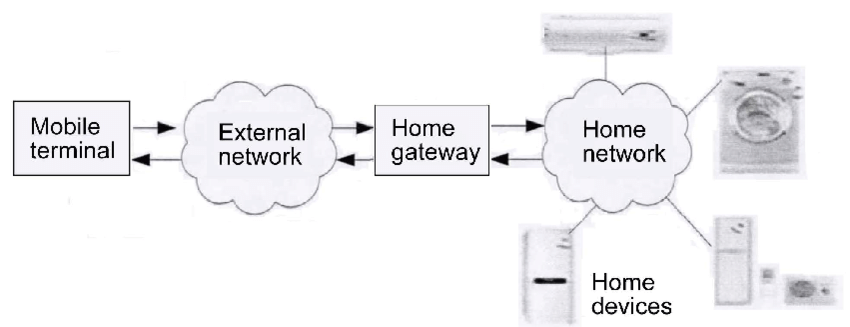
\includegraphics[width=70mm, keepaspectratio]{figures/Structure-of-smart-home-system.png}
    \caption{Okosotthoni rendszer felépítése}
\end{figure}
Mindezek a tárgyak csatlakoznak az otthoni hálózathoz, hogy megadják az állapotukat, vagy utasításokat kapjanak és vezérelhetőek legyen távolról. Az otthoni hálózat lehetővé teszi, hogy az otthon teljes mértékben összekapcsolódjon, mind külsőleg, mind belsőleg vezérelve. Az otthoni hálózati átjáró (gateaway) biztosítja a külső hozzáférést Ethernet vagy az interneten keresztül. Ez az átjáró lehetővé teszi az otthoni csatlakozást és az új szolgáltatások letöltését. A szolgáltató felelős az új szolgáltatásokért és azok elérhetőségéért a lakók számára.\cite{ricquebourg2006smart}

\section{IoT alapú intelligens otthon kialakítása}
Annak elérése érdekében, hogy minden eszköz kapcsolatban álljon egymással az általunk tervezett intelligens otthoni rendszernek a ZIGBEE-t kell hogy használja a helyi otthoni hálózat kiépítéséhez, hogy érzékelje az otthonban lévő tárgyakat vagy eszközöket, és a helyi otthoni hálózatot 3G-n vagy Etherneten keresztül összekapcsolja az internettel. A rendszer három rétegre oszlik: érzékelő és működtető réteg, hálózati réteg és alkalmazási réteg.


\subsection{Mi is az a Zigbee?}
A Zigbee egy vezeték nélküli kommunikációs forma, amelynek az alapja az IEEE 802.15.4 hálózati szabvány, ami a személyi hálózatot használja. Ez technológia több mint egy évtizede jelen van a piacon és sokan a Wi-Fi és a Bluetooth technológia alternatívájaként tekintik az alacsony fogyasztású, nagy sávszélességet nem igénylő eszközök számára.
Kiváló példa a működésének bemutatásához, hogy amikor van egy intelligens izzó és egy villanykapcsoló, amit szeretnénk összekapcsolni, hogy a kapcsolóval tudjuk irányítani az izzót. A Zigbee kommunikáció segítségével a két eszközt össze tudjuk hangolni, hogy megértsék egymást, még akkor is, ha azok teljesen más gyártótól származnak.
\par A Zigbee-t erdetileg nem P2P kommunikációra tervezték, mint például a Bluetooth-t, használatához mindenképpen szükség van egy helyben felszerelt központi egységre, egy hubra vagy átjáróra, amellyel minden eszköz tud kommunikálni.
A Zigbee további előnye, hogy egy tisztán Zigbee-alapú rendszerben csak a hub / gateway rendelkezik WiFi vagy vezetékes internetkapcsolattal, így a sok okoseszköz nem terheli túl a WiFi hálózatot, mivel minden eszköz egy dedikált rendszerben beszél egymással az okoseszközök számára, amelyek a WiFi-től eltérő frekvenciasávokat használnak, így még néhány hubdal is kiváló rendszer lehet egy nagy ingatlanban.
\par Be kell vallani, hogy a Zigbee igénytelen, egyszerű, viszont megbízható és kiválóan működik, ha intelligens rendszer kialakításához szeretnénk összekötni eszközöket.\cite{4127535}

\subsubsection{}
